\documentclass[a4paper,10pt,oneside,twocolumn,notitlepage,final]{jarticle}
\usepackage{ss20_UTF-8}

\usepackage[dvipdfmx]{graphicx}
\newcommand{\subrm}[1]{_{\mathrm{#1}}}
\newcommand{\suprm}[1]{^{\mathrm{#1}}}

\author{谷口 暁星(名古屋大学大学院 理学研究科)}
\title{データ科学的装置開発によるサブミリ波分光観測の高感度化}

\begin{document}

\abst{%
本講演では、観測データが持つ統計的な性質に注目して観測や解析の方法をデザインし直すことで、ソフトウェアの面からミリ波・サブミリ波分光観測の感度向上を目指す「データ科学的装置開発」の概要と成果を発表する。
ミリ波・サブミリ波は、ダストによる減光を受けずに分子・原子ガスの分光観測が可能な波長帯として、近傍から遠方宇宙にわたる星形成活動の研究に使われている。
ALMA望遠鏡(干渉計)による高感度・高空間分解能を生かした個別天体の観測成果は今や枚挙にいとまがない。
一方、空間・周波数の3次元空間の大規模探査による普遍的な星形成史の解明のためには、干渉計では難しい広視野観測が可能な単一望遠鏡(単一鏡)の役割が重要となる。
現在、口径50m級の次世代単一鏡計画(LST・AtLASTなど)や、超広帯域の分光装置開発(DESHIMA・SuperSpecなど)が精力的に進められている。
ところが、単一鏡の分光観測やデータ解析の方法論は、電波天文学が誕生した約半世紀前からほとんど検討・改善がなされていない。
特に、同波長帯では地球大気の熱放射の除去が問題となるが、従来の除去方法を使った観測では、装置が本来達成可能な感度を未だ実現できずにいる。
そこで我々は、単一鏡分光観測の時間$\times$周波数の行列データにおいて、大気放射が周波数方向に相関する性質(低ランク性)や、天体信号がデータに占める割合が小さい性質(スパース性)を利用した大気放射の除去手法を開発した。
低ランク性を利用した周波数変調観測では、従来のポジションスイッチ観測に比べて1/3の観測時間で同等の感度を達成できることを示した。
さらに、スパース性を利用した解析では、従来観測の取得済みデータの感度をも$\sqrt{2}$倍向上できることを示した。
}

\section{Introduction}

138億年の宇宙史において星形成活動がどのように始まり、変化を経て現在に至ったのか。
これらを解き明かすことは銀河の形成進化を理解する上で極めて重要である。
ところが、$z\gtrsim4$の初期宇宙における星形成活動の役割は、多波長観測により宇宙の星形成率密度の変遷が測定される現在でも依然として解明されていない。
この原因として、赤方偏移の決定精度が悪いこと、銀河の統計的サンプル数が圧倒的に不足していることが挙げられる。

こうした背景から、分子や電離原子の輝線を使った分光学的な赤方偏移決定に基づく、ダストの吸収を受けにくいサブミリ波による初期宇宙の分光探査が有力視されている。
明るい銀河に対しては、ALMA望遠鏡による輝線検出による分光探査の方法論が確立しつつある。
それでも干渉計であるALMA望遠鏡では視野や分光帯域が狭く一般的な明るさの銀河の観測は難しいため、星形成活動を明らかにするために十分な数の測定は得られない。
そこで、空間・周波数の3次元の宇宙論的体積を無バイアスに分光探査する、広視野のアンテナと広帯域の分光撮像装置を搭載した口径50mクラスの地上大型サブミリ波単一望遠鏡(単一鏡)が現在計画されている。

多くの開発研究を通して、ハードウェアの技術的課題は実用化の目途が立っている。
一方、ソフトウェア(観測・解析手法)の課題はまだ十分には解決の目途が立っていない。
地上のサブミリ波望遠鏡による天体検出は、同波長帯で非常に明るい地球大気の放射との闘いである。
特に主成分である水蒸気は風に乗って空間的・時間的に変動するため、観測時・解析時の大気のモデリングは必須であり、不正確なモデルは観測装置が持つ感度以上に輝線の検出を制限する原因にすらなる。
にもかかわらず、大気のモデリングの方法論は驚くべきことに電波天文学が誕生した約半世紀前からほとんど改善されておらず、ハードウェアに合わせたソフトウェアの不在が分光探査の最大のボトルネックとなっているのである。

\begin{figure*}[t]
    \centering
    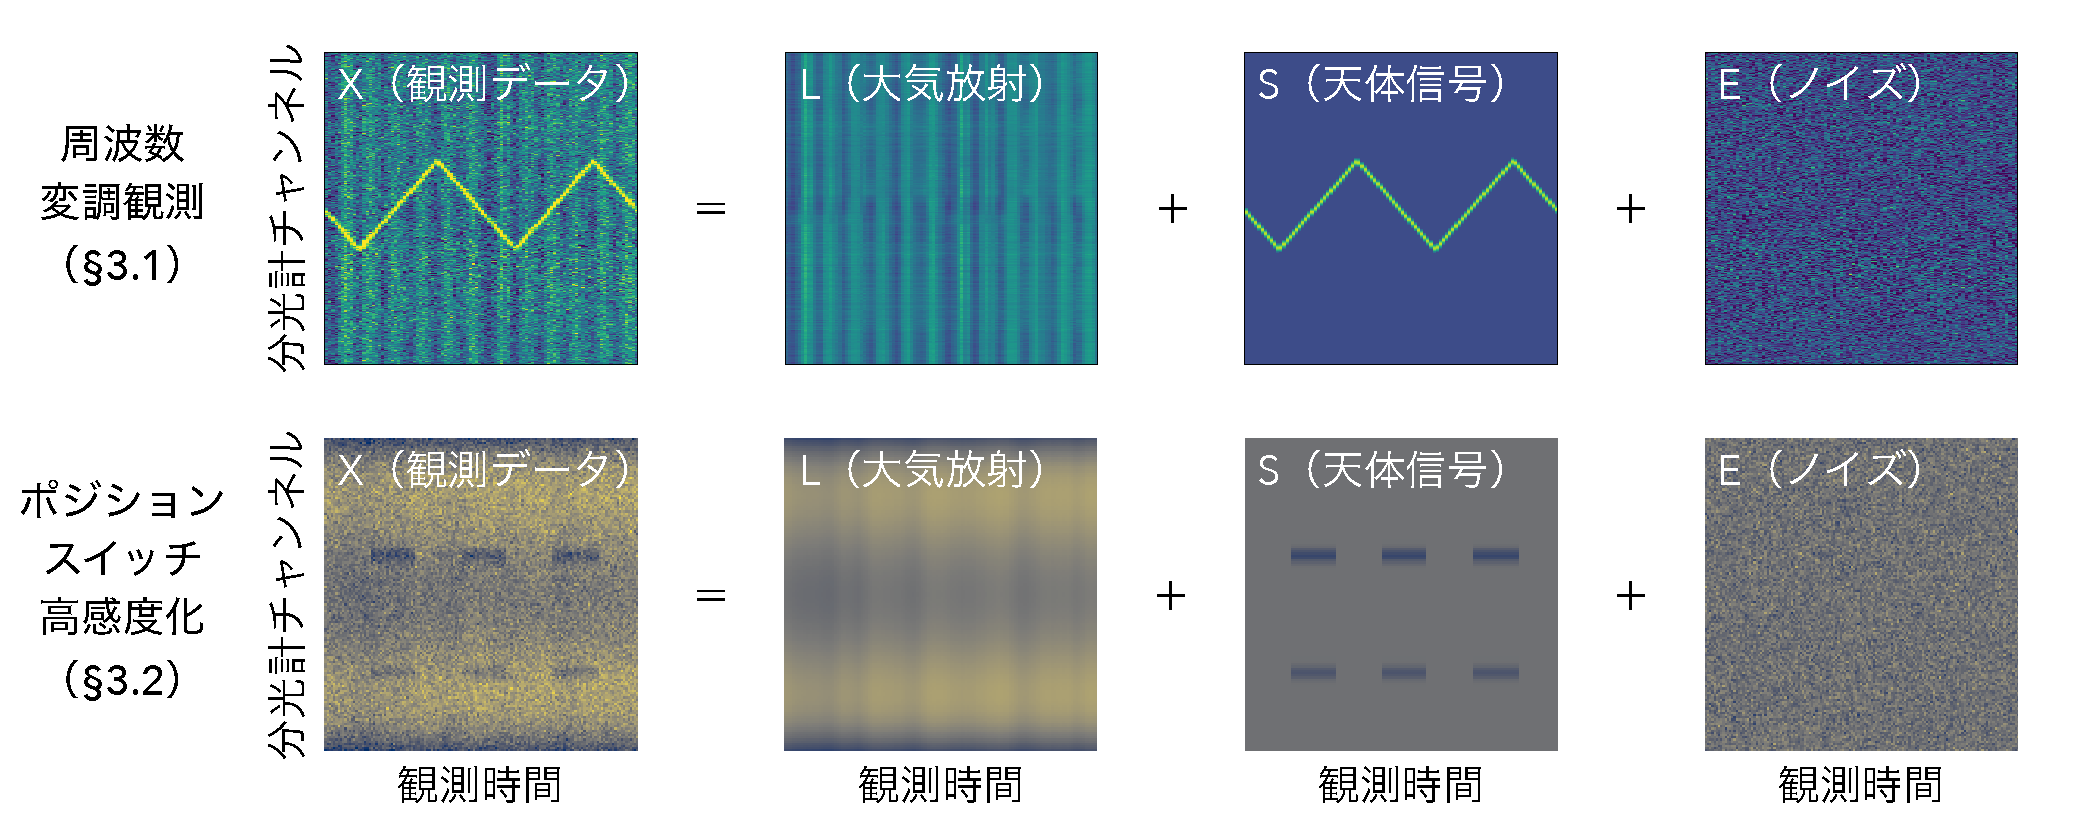
\includegraphics[width=\textwidth]{figures/figure-1}
    \caption{
        データ科学的方法に基づく2種類の単一鏡分光観測・解析手法の原理。
        時系列行列データ($X$)は0.1-1~sの高頻度で取得されるとともに、天体信号スペクトルが空間または周波数的に変調されている。
        行列分解によって低ランクの大気放射($L$)、天体信号($S$)、ノイズ($E$)成分に分解される。
        最終的なスペクトルは、$X-L$を時間方向に積分することにより得られる。
    }
    \label{fig:1}
\end{figure*}

本講演では、観測データが持つ統計的な性質に注目して観測や解析の方法をデザインし直すことで、ソフトウェアの面からミリ波・サブミリ波分光観測の感度向上を目指す「データ科学的装置開発」の概要と成果を発表する。
\ref{s:methods}節では、現在最も一般的に用いられる観測手法であるポジションスイッチ観測の問題点とデータ科学的方法に基づく解決策を提案する。
\ref{s:results}節では、データ科学的方法に基づく2種類の観測・解析手法を紹介し、実観測データへ適用することで感度の向上を実証する。
最後に、\ref{s:discussion}節で手法の応用範囲や将来計画に対する展望を議論する。

\section{Methods}
\label{s:methods}

\subsection{ポジションスイッチ観測と問題点}

ポジションスイッチ(PSW)観測は、観測天体の座標(ON点)と別の座標(OFF点)を交互に観測し、得られたスペクトル同士を減算することで、観測信号から地球大気放射を除去する手法である\citep{Wilson+13}。
観測感度$\Delta T$は以下の通りに表される。
\begin{equation}
    \Delta T
    \simeq\frac{\sqrt{2}\,T\subrm{sys}}{\sqrt{\Delta\nu\, t\subrm{total}\, \eta\subrm{obs}}}.
    \label{eq:psw-sensitivity}
\end{equation}
ここで$T\subrm{sys}$はシステム雑音温度、$\Delta\nu$は分光計の周波数分解能、$t\subrm{total}$は総観測時間、$\eta\subrm{obs}$は総観測時間に対するON点観測時間の割合(観測効率)である。
ポジションスイッチ観測は観測・解析手法として簡便なため、多くの単一鏡で天体の一点観測に現在も用いられている。
また、単一鏡によるマッピング観測でも同様にスペクトル同士の減算による大気除去が行われている。
一方、以下に列挙した問題点により、観測装置が本来持つ感度よりも観測感度が大きく低下することが知られている。

\begin{itemize}
    \item ON・OFF点のスペクトルは共に熱雑音を含むため、減算によってノイズレベルが$\sqrt{2}$倍悪化する(そのため式\ref{eq:psw-sensitivity}の分子に$\sqrt{2}$が現れる)
    \item 時間・空間的に異なる大気成分同士の減算を行うため、大気の変動をキャンセルできなかった場合、スペクトルのベースラインがうねる(実効的なノイズレベルを悪化させる)
    \item ON・OFF点を同じ割合で観測する必要があるため、観測効率が低い(望遠鏡の2点間の移動時間も考慮すると、$\eta\subrm{obs}<0.5$となる)
\end{itemize}

\begin{figure*}[t]
    \centering
    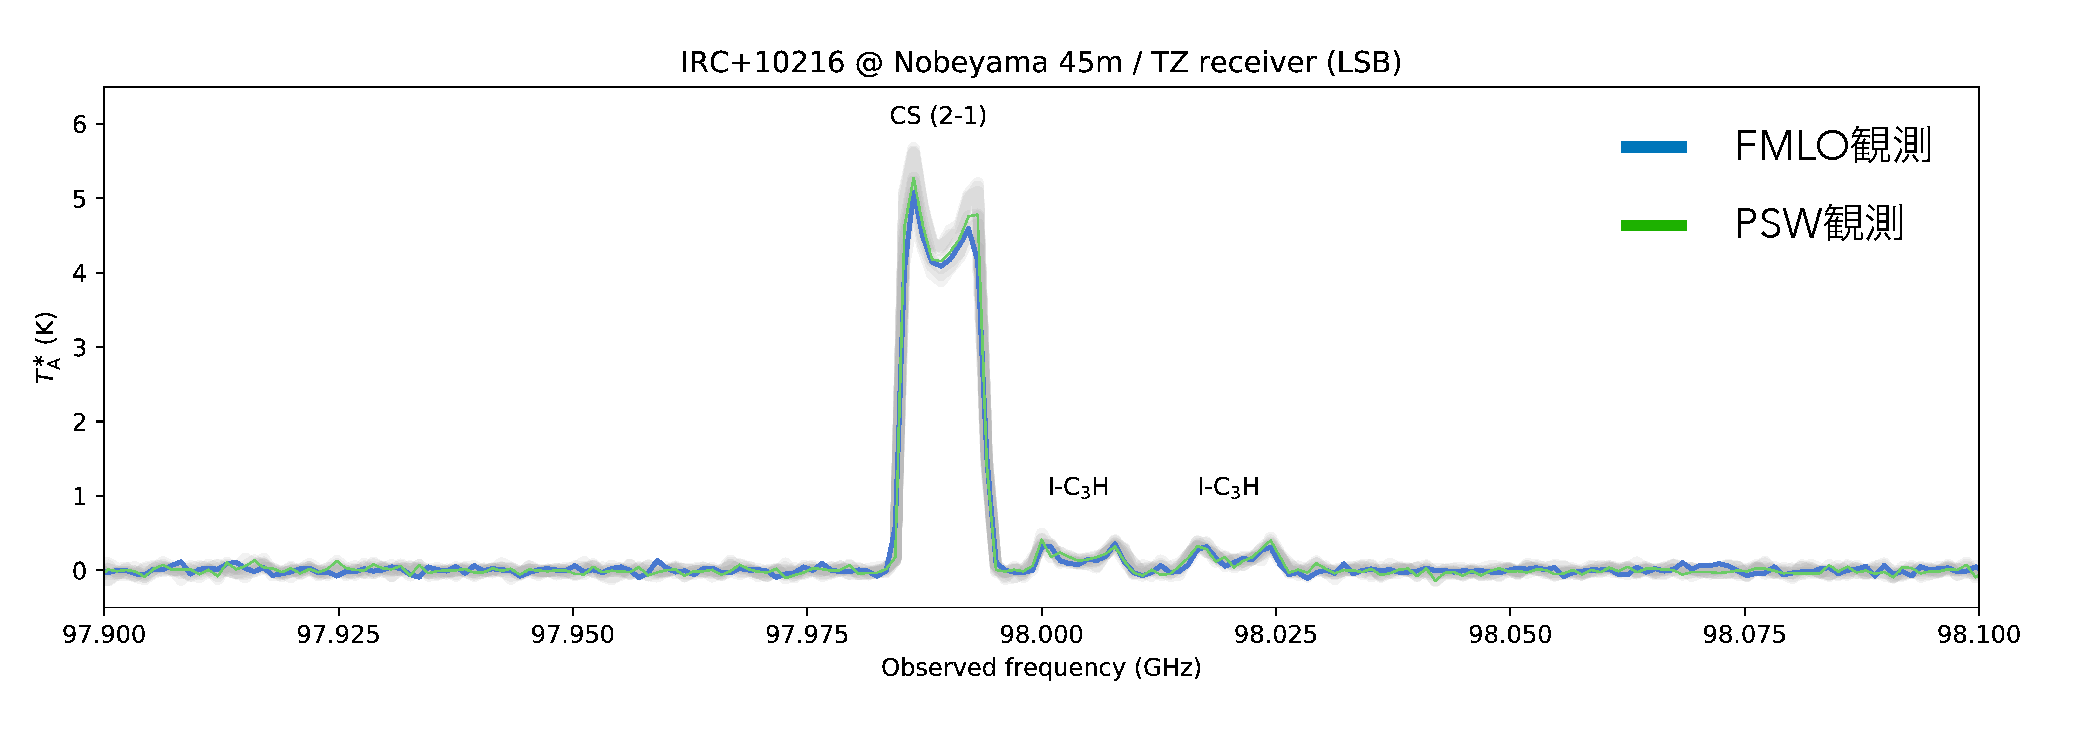
\includegraphics[width=\textwidth]{figures/figure-2}
    \caption{
        野辺山~45~m鏡・TZ受信機による、周波数変調(FMLO法)を用いた系内天体IRC+10216のCS J=2-1輝線の観測とPSW観測との比較\citep{Taniguchi+20}。
        約3倍の観測効率の向上を達成した。
    }
    \label{fig:2}
\end{figure*}

\subsection{データ科学的方法に基づく観測手法}

PSW観測(従来手法)の問題点は、大気除去のために観測データ同士の減算を行う必要がある点に集約されると言って良い。
そこで、減算を行うことなく大気放射を推定することができれば、(観測効率を除く)問題点を解決できることになるだろう。
これを実現するため、我々はデータ科学的手法に基づく新たな分光観測手法を提案する。
従来手法と比較した際の要素技術は以下に列挙した3点である。

\begin{description}
    \item[高頻度かつ連続的なデータの取得] 大気の時間変動をトレースするため、PSW観測のデータ取得間隔(典型的に1-10~s)よりも高頻度(0.1-1~s)に分光スペクトルデータを取得する。これを、時間$\times$周波数の時系列行列データとして保存する。
    \item[天体信号の変調] 統計的手法を適用するため、時系列行列データ中で天体信号成分が連続的にならないように観測方法を工夫する。これを天体信号の変調と呼ぶ(\ref{s:results}節で実際の例を紹介する)。
    \item[統計的手法による大気・天体信号の分離] 天体信号が変調された時系列行列データを用いることで、時間的・周波数的に相関を持って変動する大気成分のみからなる低ランク行列を、行列分解の統計的手法を使って推定する。
\end{description}

図\ref{fig:1}に、変調方法の異なる2つの観測手法によって得られた時系列行列データから、それぞれ大気成分を分離する様子を示した。
従来手法と異なり、減算は観測行列とノイズをほとんど含まない推定行列同士で行われるため、ノイズレベルの$\sqrt{2}$倍の悪化が発生しないことが期待される。
また、大気の時間変動をリアルタイムで推定することにより、ベースラインのうねりも発生しにくいことが利点である。

\section{Results}
\label{s:results}

\subsection{周波数変調を使ったオフ点不要の高効率な分光観測手法}

ヘテロダイン受信機を使った観測では、局部発振器(LO)の周波数を変えることで観測周波数帯を観測中に容易に動かすことができる。
我々はこれを応用し、高頻度($\sim10$~Hz)なデータ取得と同時に天体信号を周波数方向に変調(FM)させることで、データ科学的方法を応用可能にした周波数変調観測手法(FMLO法)を開発した\citep{Taniguchi+20}。
\ref{s:methods}節で示した利点に加え、FMLO法はOFF点を観測する必要がないため、高い観測効率($\eta\subrm{obs}>0.9$)を達成可能である。
図\ref{fig:2}に示した野辺山 45~m 鏡における試験観測では、PSW観測の1/3の観測時間で同等の観測感度を達成できることを実証した。
これは、式\ref{eq:psw-sensitivity}において、$\sqrt{2}\rightarrow1.1$、$\eta\subrm{obs}=0.92$の改善が達成されたことに対応する。

\begin{figure*}[t]
    \centering
    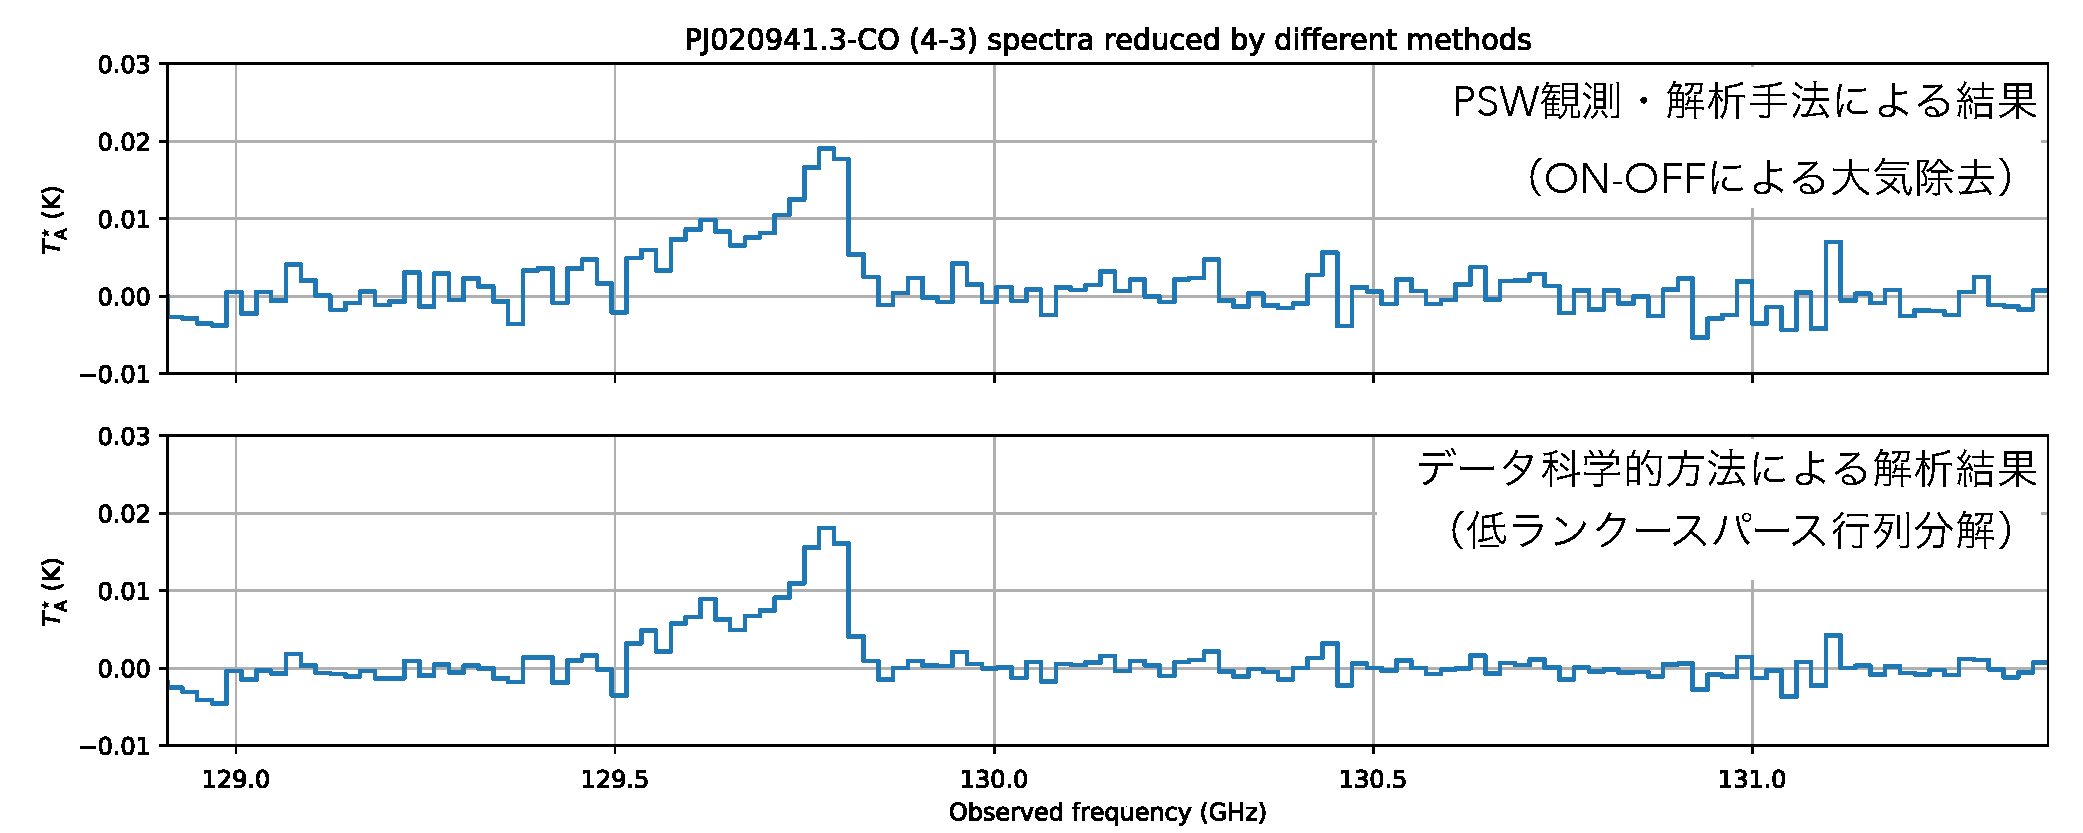
\includegraphics[width=\textwidth]{figures/figure-3}
    \caption{
        メキシコLMT~50~m鏡・B4R受信機による、高赤方偏移銀河PJ020941.3のCO J=4-3輝線のPSW観測を従来・提案手法で解析した結果。
        スイッチングは10~s間隔、データは1~s間隔で取得されている。
    }
    \label{fig:3}
\end{figure*}

\subsection{ポジションスイッチ観測の高感度化}

PSW観測のスイッチング間隔よりも高頻度($>1$~Hz)でデータ取得ができれば、スイッチングそのものを天体信号の変調とみなしてデータ科学的方法を適用できる。
特に、高赤方偏移銀河のように輝線が1-2本程度しか検出されない場合、天体信号は行列中でスパース(非ゼロの要素が少ない)となるため、低ランク--スパース行列分解手法\citep{Thou+11}を利用して大気の分離が可能である。
図\ref{fig:3}に示したメキシコLMT 50~m 鏡・B4R受信機(Kawabe et al. in prep)による試験観測では、PSW観測の1.65倍の感度を達成可能であることを実証した(Taniguchi et al. in prep)。
これは、$\sqrt{2}\rightarrow1$に加え、ベースラインのうねりを除去できたことを意味する。

\section{Discussion}
\label{s:discussion}

\ref{s:results}節で実証した2種類の観測・解析手法は、ハードウェアの大規模な追加開発を必要とすることなく、既存の単一鏡の感度の向上が可能である。
FMLO法はこれに加え、OFF点のコンタミネーション(OFF点に天体信号が存在していた場合、ON点の天体信号の強度が低く推定される問題)が原理的に発生しないため、ALMAのTotal Power Arrayのような高感度な単一鏡への応用が期待される。

ポジションスイッチ観測の高感度化は、高頻度なデータ取得が可能であれば追加の開発が不要なばかりか、既存の観測データの感度さえも向上できる可能性を秘めている。
また、DESHIMA\citep{Endo+19b}のような、近年開発が進む超広帯域フィルターバンク分光計(原理的に周波数変調が不可能な装置)との相性も良い。
観測装置の特性を理解し、観測・解析手法を使い分けていくことが今後重要となるだろう。

\section{Conclusions}
\label{s:conclusions}

本研究によって、データ科学的手法を単一鏡の分光観測に適用するための方法論が確立され、開発した2種類の観測・解析手法によって、ソフトウェア開発で観測感度を向上できることが実証された。
ハードウェア開発に並ぶ第二の開発領域として、将来計画を牽引するための技術的な目処が立ったと言える。

\small
\begin{thebibliography}{99}
    \bibitem[Endo et~al. (2019b)]{Endo+19b}
    Endo, A., et al. 2019, Nature Astronomy, 3, 989
    \bibitem[Taniguchi et~al. (2020)]{Taniguchi+20}
    Taniguchi, A., et al. 2020, PASJ, 72, 2
    \bibitem[Thou \& Tao (2011)]{Thou+11}
    Thou, T., \& Tao, D. 2011, ICML-11, 33
    \bibitem[Wilson et~al. (2013)]{Wilson+13}
    Wilson, T.~L., Rohlfs, K., \& H\"{u}ttemeister, S. 2013, Tools of Radio Astronomy Sixth Edition
\end{thebibliography}
\end{document}
